\documentclass{beamer}
\usepackage{graphicx}
\usepackage{hyperref}

% Set transparency of non-highlighted sections in the table of
% contents slide.
\setbeamertemplate{section in toc shaded}[default][100]
\AtBeginSection[]
{
  \setbeamercolor{section in toc}{fg=red} 
  \setbeamercolor{section in toc shaded}{fg=black} 
  \begin{frame}
    \tableofcontents[currentsection]
  \end{frame}
}

\begin{document}

\title{R project in Google Summer of Code}

\author{
  Toby Dylan Hocking\\
  toby.hocking@mail.mcgill.ca}

\date{12 April 2016}

\maketitle

\begin{frame}
  \frametitle{R is a free/open-source software environment for
    statistics and graphics}
  \begin{itemize}
  \item \url{https://www.r-project.org/} 
\includegraphics[width=1cm]{Rlogo}
  \item A command interpreter for the R programming language.
  \item Packages for machine learning, data analysis, visualization.
  \item Completely free and open for anyone to use and modify\\(GNU
    General Public License version 2).
  \end{itemize}
  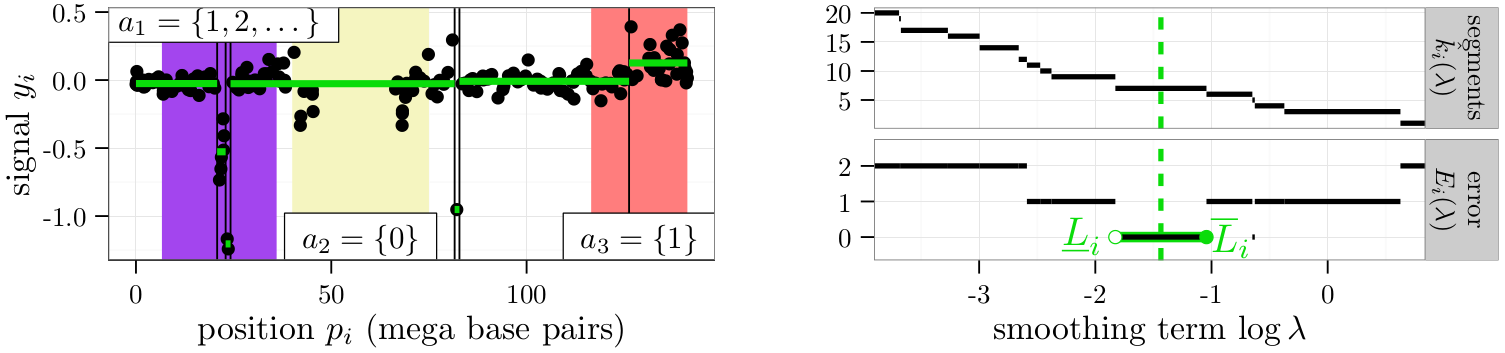
\includegraphics[width=\textwidth]{HOCKING-ICML2013-Figure1}
  
  Figure source: Hocking et al, ``Learning sparse penalties for
  change-point detection using max-margin interval regression,''
  International Conference on Machine Learning 2013.
\end{frame}

% \begin{frame}[fragile]
% \frametitle{Brief demo of R}
%   \scriptsize
% \begin{verbatim}
% thocking@silene:~/R/gsoc2016(master*)$ R --vanilla

% R version 3.2.3 (2015-12-10) -- "Wooden Christmas-Tree"
% Copyright (C) 2015 The R Foundation for Statistical Computing
% Platform: x86_64-pc-linux-gnu (64-bit)

% R is free software and comes with ABSOLUTELY NO WARRANTY.
% You are welcome to redistribute it under certain conditions.
% Type 'license()' or 'licence()' for distribution details.

%   Natural language support but running in an English locale

% R is a collaborative project with many contributors.
% Type 'contributors()' for more information and
% 'citation()' on how to cite R or R packages in publications.

% Type 'demo()' for some demos, 'help()' for on-line help, or
% 'help.start()' for an HTML browser interface to help.
% Type 'q()' to quit R.

% > 
% \end{verbatim}
% \end{frame}

\begin{frame}
  \frametitle{History of R project and Google Summer of Code}
  \begin{description}
  \item[1992] First \textbf{R} coded by Robert Gentleman and Ross
    Ihaka at University of Auckland, New Zealand.
  \item[1997] First Comprehensive R Archive Network (CRAN) web site
    hosting \textbf{R packages}.
  \item[1998] Google incorporated in Stanford, California.
  \item[2005] First \textbf{Google Summer of Code} (GSOC).
  \item[2008] First time R participates in GSOC (GSOC-R).
  \item[2012] My first year as co-administrator of GSOC-R.
  \end{description}
  Sources: Wikipedia, GSOC web site.
\end{frame}

\begin{frame}
  \frametitle{Google Summer of Code (GSOC)}
Student gets \$5500 for writing open source code for
    3 months.
    \begin{description}
    \item[Feb] \textbf{Admins} for open source organizations
      e.g. R, Debian, Wikimedia, Mozilla, apply to Google.
    \item[Mar] \textbf{Mentors} suggest projects for each org.\\
      \textbf{Students} submit project proposals to Google.\\
      Google gives funding for $n$ students to an org.
    \item[April] The top $n$ students get \$500 and begin coding.
    \item[July] Midterm evaluation, pass = \$2250.
    \item[Aug] Final evaluation, pass = \$2750.
    \item[November] Orgs get \$500/student mentored.
    \end{description}
  I have participated as an \textbf{admin} and \textbf{mentor} for the
  R project.
\end{frame}

\begin{frame}[fragile]
  \frametitle{Student projects in R Google Summer of Code}
  \begin{tabular}{ccc}
    year & total students & students I mentored \\
    \hline
    2008 & 4 \\
    2009 & 4 \\
    2010 & 5 \\
    2011 & 15 \\
    2012 & 16 \\
    2013 & 18 & 1\\
    2014 & 17 & 1\\
    2015 & 23 & 3 
  \end{tabular}
\end{frame}

\begin{frame}
  \frametitle{What makes a good GSOC project?}
  Coding projects should:
  \begin{itemize}
  \item Result in free/open-source software.
  \item Be 3 months of full time work for a student.
  \item Include writing documentation and tests.
  \item Not include original research.
  \end{itemize}
  Examples: 
  \begin{itemize}
  \item Write a new R package.
  \item Improve an existing R package.
  \end{itemize}  
\end{frame}


\begin{frame}[fragile]
\frametitle{Example: R package animint, 2013--present}
\begin{itemize}
  \item Useful for interactive data visualization, for example
    {\small \url{http://bl.ocks.org/tdhock/raw/10f27e4ace80bffa10a0/}}\\
    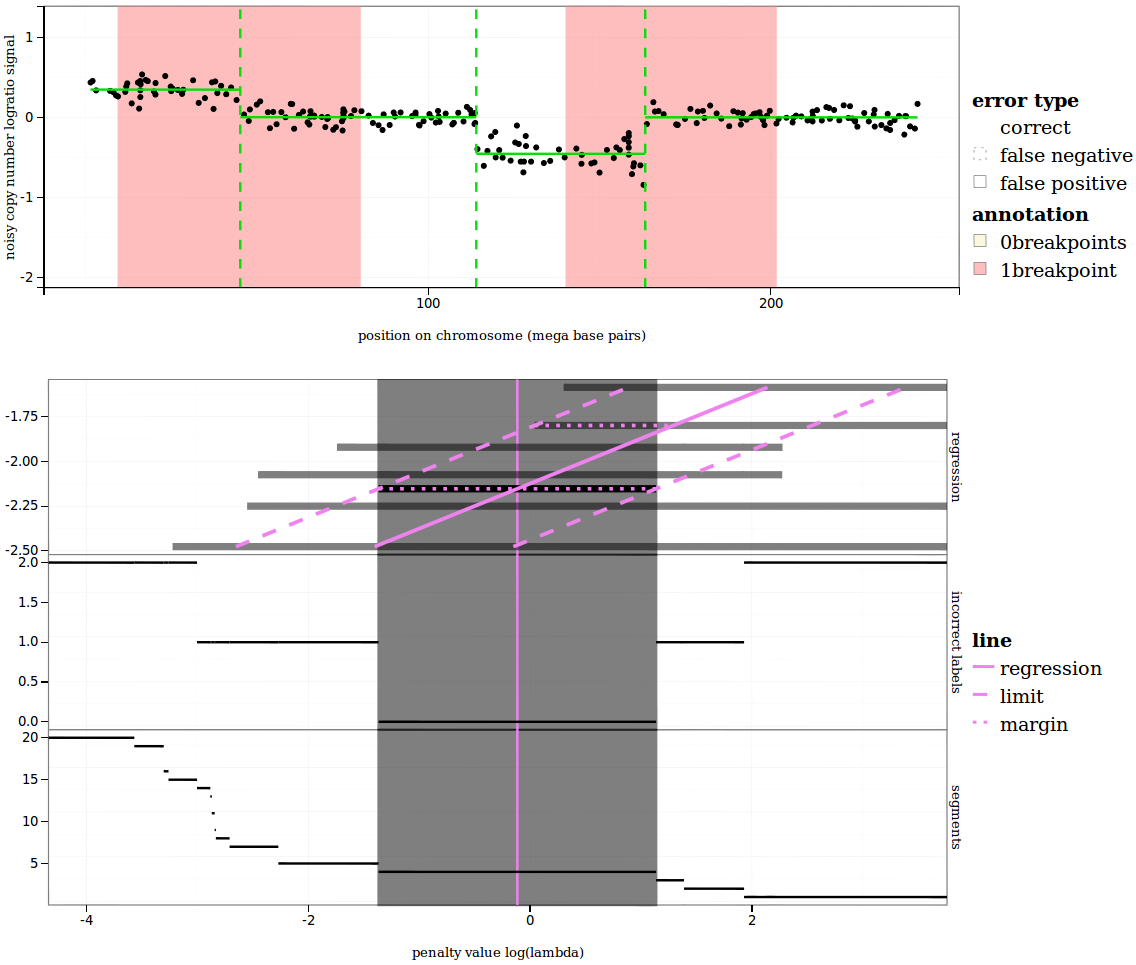
\includegraphics[width=0.5\textwidth]{screenshot-max-margin-interval-regression}
  %\item \url{https://github.com/tdhock/animint}
  \item Students I mentored:
    \begin{tabular}{cccc}
      Student & Country & Year & Features coded \\
      \hline
      Susan VanderPlas & USA & 2013 & Legends, geoms. \\
      Carson Sievert & USA & 2014 & Tests, facets, etc. \\ 
      Tony Tsai & China & 2015 & Efficient compilation.\\
    \end{tabular}
\end{itemize}
\end{frame}

\end{document}
